\chapter{Approach}
\label{ch:approach}
%%%%%%%%%%%%%%%%%%%%%%%
% - description of the designed system
% - analysis and review of the current software architecture
%%%%%%%%%%%%%%%%%%%%%%%


The basic architecture pattern of the Basilisk platform is the microservice architecture (see chapter \ref{sec:microservice_architecture} for a short description). 
This means that the platform is dividable into multiple parts which could run on different hardware systems.

There are three main services.
These services communicate via message queues.


The Hooks Checking Service which regularly polls the Github or Dockerhub repositories for new versions of the observed \tsp{}.
The Jobs Managing Service processes the requests coming from the web-frontend, checks if the Hooks Checking Service has found a new version for a benchmark and creates jobs for new benchmarks.
Lastly the \ts{} Benchmarking Service executes the benchmarks given to it and saves the results to a database.

The services will be deeper explained in the following sections.



\begin{figure}[tbph]
	\centering
	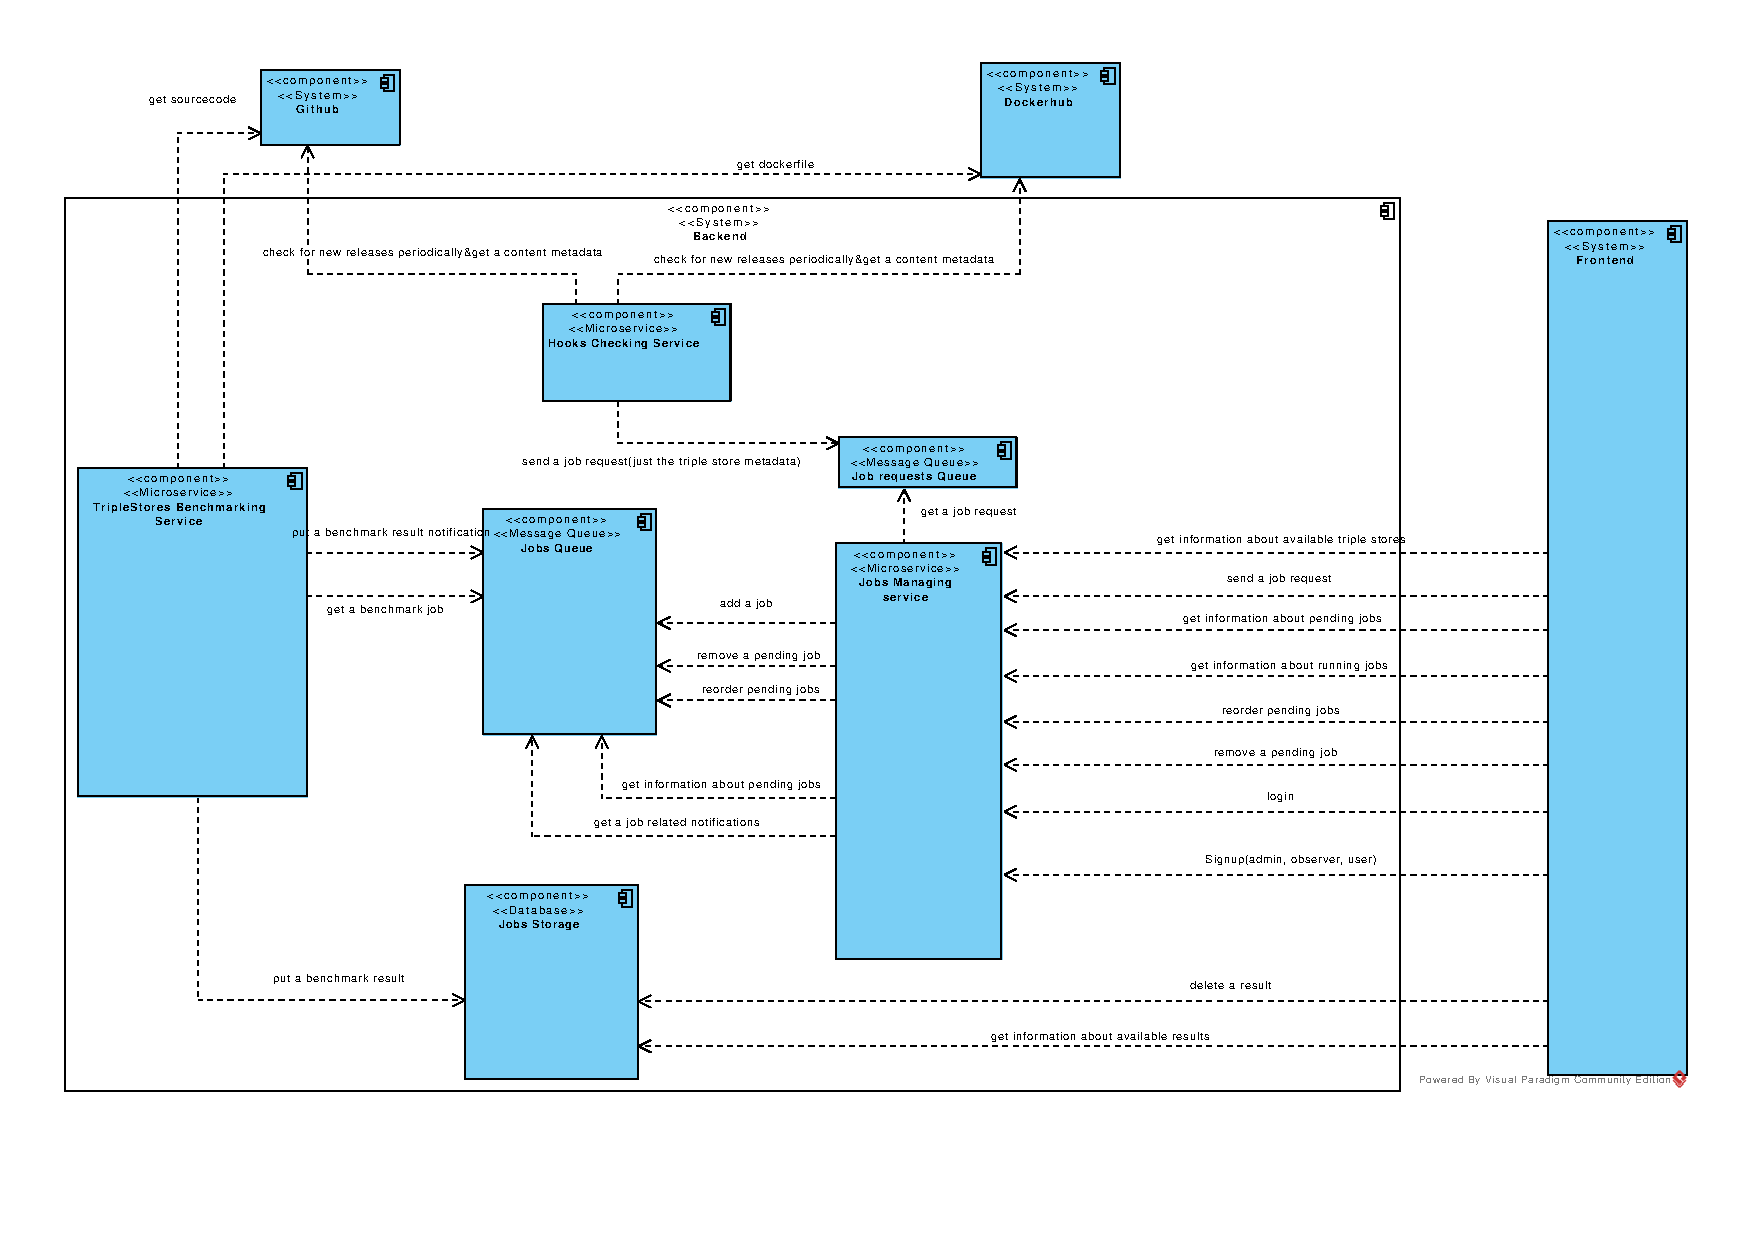
\includegraphics[width=1.1\textwidth]{figures/basilisk_high_level_design.pdf}
	\caption{High level design of the Basilisk framework}
	\label{fig:basilisk_high_level_design}
\end{figure}
